
\chapter[Dạng bài: Xác định điểm có pha dao động thỏa mãn điều kiện cho trước]{Dạng bài: Xác định điểm có pha dao động thỏa mãn điều kiện cho trước}
\section{Lý thuyết}
\subsection{Nếu hai nguồn cùng pha}
\begin{itemize}
	\item M dao động cùng pha với nguồn khi $d=k\lambda$.
	
	\item M dao động ngược pha với nguồn khi $d = (2k+1) \dfrac{\lambda}{2}$.
\end{itemize}	
\subsection{Nếu hai nguồn ngược pha}	\begin{itemize}
	\item M dao động cùng pha với nguồn khi $d=(2k+1) \dfrac{\lambda}{2}$.
	
	\item M dao động ngược pha với nguồn khi $d=k\lambda$. 
\end{itemize}
\section{Mục tiêu bài học - Ví dụ minh họa}
\begin{dang}{Xác định được điểm dao động cùng pha hoặc ngược pha với nguồn}
	\ppgiai{\begin{description}
			\item[Bước 1:] Xác định điều kiện về pha của điểm M, suy ra hệ thức quy định giá trị của $k$. 
			\item[Bước 2:] Lựa chọn giá trị $k$ ứng với điểm M phù hợp với yêu cầu của đề bài.
	\end{description}}
	\viduii{3}{Trên mặt nước có 2 nguồn sóng giống hệt nhau A và B cách nhau một khoảng AB = 24 cm. Bước sóng $\lambda = \text{2,5}\ \text{cm}$. Hai điểm M và N trên mặt nước cùng cách đều trung điểm của đoạn AB một đoạn 16 cm  và cùng cách đều 2 nguồn sóng và A và B. Số điểm trên đoạn MN dao động cùng pha với 2 nguồn là  
		\begin{mcq}(4)
			\item 4.                         
			\item 8.                               
			\item 6.                              
			\item 9.
		\end{mcq}
	}
	{
		\begin{center}
			\textbf{Hướng dẫn giải}
		\end{center}
		
		\begin{itemize}
			\item  Gọi M là điểm dao động cùng pha với nguồn.
			\item Phương trình sóng tổng hợp tại M là
			
			\begin{equation*}
				u_{\text{M}} = 2a \cos \left(\pi \dfrac{d_2-d_1}{\lambda}\right) \cos \left( 20\pi t - \pi \dfrac{d_2+d_1}{\lambda}\right).
			\end{equation*}
			\item Để M dao động ngược pha với $\text{S}_1$ thì
			\begin{equation*}
				\pi \dfrac{d_2+d_1}{\lambda} =2k\pi,
			\end{equation*}
			suy ra $d_2+d_1=2k\lambda$.
			\item Với $d_1=d_2$ ta có $d_2=d_1=k\lambda$.
			Gọi $x$ là khoảng cách từ M đến AB 
			\begin{equation*}
				d_1=d_2 =\sqrt {x^2 + \left(\dfrac{AB}{2}\right)^2} =k\lambda. 
			\end{equation*}
			\item Suy ra 
			\begin{equation*}
				|x|=\sqrt {(k\lambda)^2 - \left(\dfrac{AB}{2}\right)^2}=\sqrt {\text{6,25}k^2-144}.
			\end{equation*}
			\item Với:
			\begin{equation*}
				0 \leq x \leq 16 \Leftrightarrow \text{4,8} \leq k \leq 8 \Rightarrow k=5; 6; 7; 8.
			\end{equation*}
			\item Vậy trên đoạn MN có 4 điểm dao động cùng pha với hai nguồn.
		\end{itemize}
		
		\textbf{Đáp án: A.}
	}
	\viduii{3}
	{Trên mặt nước có 2 nguồn sóng giống nhau A và B cách nhau 12 cm đang dao động vuông góc với mặt nước tạo ra sóng có bước sóng 1,6 cm. Điểm C cách đều 2 nguồn và cách trung điểm O của AB một khoảng 8 cm. Số điểm dao động ngược pha với nguồn trên đoạn CO là
		
		\begin{mcq}(4)
			\item 3.
			\item 4.
			\item 5.
			\item 2.
		\end{mcq}
	}
	{\begin{center}
			\textbf{Hướng dẫn giải}
			
			\vspace*{1em}
			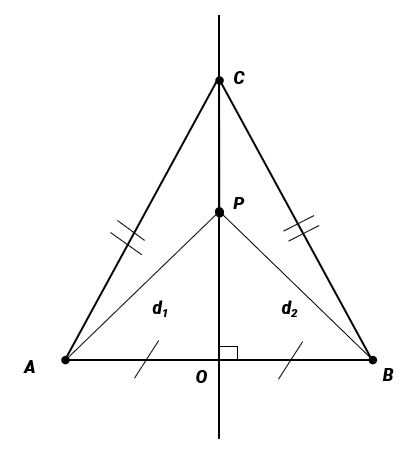
\includegraphics[scale=0.6]{../figs/VN12-PH-11-A-007-2-V2-1.JPG}
		\end{center}
		
		\begin{itemize}
			\item Giả sử điểm P trên đoạn CO cách 2 nguồn khoảng $d_1$ và $d_2$. Vì C cách đều hai nguồn nên CO là trung trực của AB. Do đó $d_1=d_2$.
			\item Giả sử phương trình sóng của hai nguồn là:
			\begin{equation*}
				u_{\text{A}}=u_{\text{B}} = a \cos \omega t.
			\end{equation*}
			\item Phương trình sóng tại P do nguồn A và nguồn B truyền tới:
			\begin{equation*}
				u_{\text{AP}}= a \cos \left(\omega t - \dfrac{2\pi d_1}{\lambda}\right) = a \cos \left(\omega t - \dfrac{2\pi d}{\lambda}\right),
			\end{equation*}
			\begin{equation*}
				u_{\text{BP}}= a \cos \left(\omega t - \dfrac{2\pi d_2}{\lambda}\right) = a \cos \left(\omega t - \dfrac{2\pi d}{\lambda}\right).
			\end{equation*}
			\item Phương trình sóng tổng hợp tại P:
			\begin{equation*}
				u_{\text{P}}=	u_{\text{AP}} + u_{\text{BP}}= a \cos \left(\omega t - \dfrac{2\pi d}{\lambda}\right) + a \cos \left(\omega t - \dfrac{2\pi d}{\lambda}\right) = 2a\cos \left(\omega t - \dfrac{2\pi d}{\lambda}\right).
			\end{equation*}
			\item Vì P dao động ngược pha so với nguồn nên độ lệch pha bằng $\pi + k2\pi$, do đó ta có:
			\begin{equation*}
				\Delta \varphi = \omega t - \left(\omega t - \dfrac{2\pi d}{\lambda}\right) =\dfrac{2\pi d}{\lambda} = \pi + k2\pi \Rightarrow \dfrac{2\pi d}{\lambda} = \pi +k2\pi \Rightarrow d = (2k+1) \dfrac{\lambda}{2}.
			\end{equation*}	
			\item Cho P chạy trên CO thì ta có AO $\leq d \leq$ AC. Từ đó
			\begin{equation*}
				\dfrac{\text{AB}}{2} \leq (2k+1) \dfrac{\lambda}{2} \leq \sqrt {\left(\dfrac{\text{AB}}{2}\right)^2 + \text{OC}^2}.
			\end{equation*}
			\item Thay số ta được $6 \leq (2k+1) \text{0,8} \leq 10 \Rightarrow \text{3,25} \leq k \leq \text{5,75}.$
			\item Suy ra $k=4$ và $k=5$.
			\item Có 2 giá trị của $k$ nên trên đoạn CO có 2 điểm dao động ngược pha với nguồn.
		\end{itemize}
		
		\textbf{Đáp án: D.}
	}
\end{dang}
\begin{dang}{Xác định được điểm dao động với biên độ cực đại (hoặc cực tiểu), đồng thời\\ cùng pha (hoặc ngược pha) với nguồn}
	\viduii{3}
	{Có hai nguồn sóng cơ kết hợp A và B trên mặt nước cách nhau một đoạn $\text{AB} = 9 \lambda$ phát ra dao động với phương trình $u=a \cos \omega t$. Xác định trên đoạn AB có bao nhiêu điểm dao động với biên độ cực đại cùng pha với hai nguồn (không kể hai nguồn).
		
		\begin{mcq}(4)
			\item 12.
			\item 6.
			\item 8.
			\item 10.
		\end{mcq}
	}
	{\begin{center}
			\textbf{Hướng dẫn giải}
			
			\vspace*{1em}
			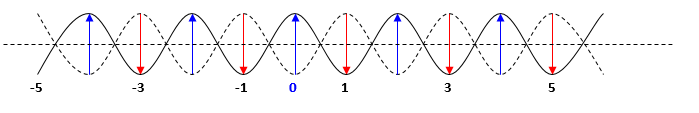
\includegraphics[scale=0.7]{../figs/VN12-PH-11-A-007-2-V2-2.png}
		\end{center}
		
		Xét điểm M trên đoạn $\text S_1 \text S_2$, với $d_1 = \text S_1 \text M$, $d_2 = \text S_2 \text M$. Ta có:
		
		$$u_\text{M} = 2a \cos \left(\dfrac{\pi (d_2 - d_1)}{\lambda}\right) \cos (\omega t - 9 \pi)$$
		
		Để M dao động với biên độ cực đại, cùng pha với hai nguồn thì:
		$$\cos \left(\dfrac{\pi (d_2 - d_1)}{\lambda}\right) = - 1 \Rightarrow \left(\dfrac{\pi (d_2 - d_1)}{\lambda}\right) = (2k + 1) \pi \Rightarrow d_2 - d_1 = (2k+1) \lambda$$
		
		Ngoài ra: $d_1 + d_2 = 9 \lambda$
		
		Vậy $d_1 = (4-k) \lambda$.
		
		Ta có:
		$$0 < (4-k) \lambda < 9 \lambda \Rightarrow -5 < k < 4$$
		
		Có 8 giá trị của $k$.
		
		\textbf{Đáp án: C.}
	}
	\viduii{3}
	{Hai nguồn phát sóng kết hợp A và B trên mặt chất lỏng dao động theo phương trình $u_\text A = a \cos 100 \pi t$ và $u_\text B = b \cos 100 \pi t$. Tốc độ truyền sóng trên mặt chất lỏng là $1\ \text{m/s}$. Gọi I là trung điểm của AB, M là điểm nằm trên đoạn AI, N là điểm nằm trên đoạn BI. Biết $\text{IM} = 5\ \text{cm}$ và $\text{IN} = 6,5\ \text{cm}$. Số điểm nằm trên đoạn MN có biên độ cực đại và cùng pha với I là
		
		\begin{mcq}(4)
			\item 7.
			\item 4.
			\item 5.
			\item 6.
		\end{mcq}
	}
	{\begin{center}
			\textbf{Hướng dẫn giải}
		\end{center}
		
		Vì hai nguồn cùng pha nên I dao động với biên độ cực đại.
		
		Những điểm cùng pha với I thì cách I một số nguyên lần bước sóng.
		
		Mà $\text{IM} = 5\ \text{cm} = 2,5 \lambda$ nên trên IM có 2 điểm. 
		
		Và $\text{IN} = 6,5\ \text{cm} = 3,25 \lambda$ nên trên IN có 3 điểm.
		
		Vậy có tổng cộng 5 điểm dao động với biên độ cực đại và cùng pha với I.
		
		\textbf{Đáp án: C.}
	}
	\viduii{4}{Ở mặt chất lỏng có hai nguồn sóng A, B cách nhau $19\ \text {cm}$, dao động theo phương thẳng đứng với phương trình $u_\text A = u_\text B = a \cos 20 \pi t$ (với $t$ tính bằng s). Tốc độ truyền sóng là $40\ \text{cm/s}$. Gọi M là điểm ở mặt chất lỏng gần A nhất sao cho phần tử chất lỏng tại M dao động với biên độ cực đại và cùng pha với nguồn. Khoảng cách AM là
		\begin{mcq}(4)
			\item 5 cm
			\item 2 cm.                               
			\item 4 cm.                              
			\item $\sqrt{2}$ cm.
		\end{mcq}
	}
	{
		\begin{center}
			\textbf{Hướng dẫn giải}
			
			\vspace*{1em}
			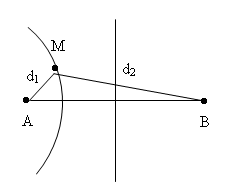
\includegraphics[scale=0.8]{../figs/VN12-PH-11-A-007-2-V2-1.png}
		\end{center}
		
		Ta có: $\lambda=\dfrac{v}{f}=4\ \text{cm}$.
		
		Số cực đại giao thoa:
		$$-\dfrac{\text{AB}}{\lambda}\leq k \leq \dfrac{\text{AB}}{\lambda} \Rightarrow k = -4; -3; \ldots ; 3; 4$$
		
		Điểm M gần A nhất dao động với biên độ cực đại thì $k=4$.
		
		Do M dao động cùng pha với nguồn nên
		$$\Delta \varphi = \dfrac{\pi (d_1 + d_2)}{\lambda} n 2 \pi \Rightarrow d_1 + d_2 = 2n\lambda = 8n\ (1)$$
		
		Mà $$d_1 + d_2 \geq \text{AB} d_1 + d_2 \geq\ (2)$$
		
		Từ (1) và (2) suy ra $$n \geq 2,375$$
		
		Vậy $n=3; 4; \ldots$.
		
		Mà M dao động với biên độ cực đại nên $d_2 - d_1=4\lambda = 16\ (3)$
		
		Từ (1), (2), (3) ta được
		$$d_1 = 4n - 8$$
		
		Vậy $d_1$ nhỏ nhất khi $n=3$, khi đó $d_1 = 4\ \text{cm}$.
		
		\textbf{Đáp án: C.}
	}
\end{dang}